\documentclass{poly}
\usepackage{main}

\title{Probabilités conditionnelles}
\author{Terminale STMG1}
\date{}

\begin{document}
\maketitle

\section{Rappels de vocabulaire}
On considère comme exemple d'expérience aléatoire le lancer d'un dé équilibré à 6 faces dont on observe le résultat.
\begin{tcolorbox}
\begin{itemize}
\item L'univers d'une expérience aléatoire, noté $\Omega$, est l'ensemble de toutes les issues possibles $\to \Omega = \{1;2;3;4;5;6\}$ dans le cas du lancer de dé.
\item Un événement est une partie de $\Omega$, c'est ce dont on va évaluer la probabilité $\to$ $A$\og Obtenir un pair\fg est un événement, de probabilité $P(A) = \dfrac{3}{6} = \dfrac{1}{2}$.
\item $\Omega$ est aussi un événement appelé \textbf{événement certain}, avec $P(\Omega) = 1$
\item Si $A$ et $B$ sont deux événements, alors la réalisation de $A$ \textbf{ou bien} de $B$ est modélisée par l'\textbf{union} $A \cup B$ $\to$ l'union de $A$\og Obtenir 2\fg et de $B$\og Obtenir 4\fg est $A \cup B$\og obtenir 2 ou 4\fg.
\item Si $A$ et $B$ sont deux événements, alors la réalisation de $A$ \textbf{et} de $B$ est modélisée par l'\textbf{intersection} $A \cap B$ $\to$ l'intersection de $A$\og Obtenir un pair\fg et de $B$\og Obtenir un $2$ ou un $3$\fg est $A \cap B$\og Obtenir un $2$\fg
\end{itemize}
\end{tcolorbox}

\newpage
\section{Représentation d'expérience aléatoire}
\begin{example}
Soit une expérience aléatoire d'univers $\Omega$, et deux événements $A$ et $B$ d'$\Omega$. Alors, l'arbre pondéré suivant donne le moyen de calculer certaines probabilités.
\begin{center}
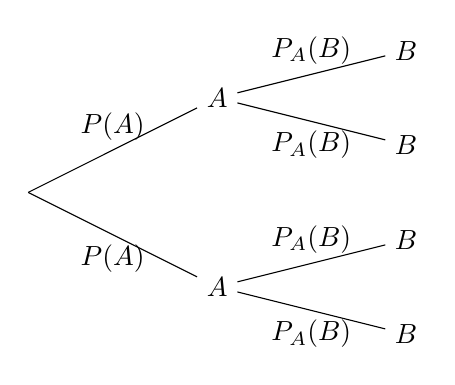
\begin{tikzpicture}[scale=1.2]
\node (A) at (2,1) {$A$};
\node (AB) at (4,1.5) {$B$};
\node (ABn) at (4,0.5) {$\overbar{B}$};
\node (An) at (2,-1) {$\overbar{A}$};
\node (AnB) at (4,-0.5) {$B$};
\node (AnBn) at (4,-1.5) {$\overbar{B}$};
\draw (0,0) -- (A) node[above,midway] {$P(A)$} -- (AB) node[midway,above] {$P_A(B)$};
\draw (A) -- (ABn) node[midway,below] {$P_A(\overbar{B})$};
\draw (0,0) -- (An) node[midway,below] {$P(\overbar{A})$} -- (AnB) node[above,midway] {$P_{\overbar{A}}(B)$};
\draw (An) -- (AnBn) node[below,midway] {$P_{\overbar{A}}(\overbar{B})$};    
\end{tikzpicture}
\end{center}
\end{example}
\begin{proposition}
\hfill
\begin{itemize}
\item Une branche de la racine à une extrémité correspond à l'intersection des événements correspondants. Pour calculer la probabilité de cette intersection, il faut multiplier les probabilités sur la branche.
\item La somme de toutes les probabilités issues d'un même noeud vaut $1$.
\item La probabilité d'un événement est égale à la somme des probabilités de toutes les branches contenant cet événement. 
\end{itemize}        
\end{proposition}
\begin{exercize}
Soit une urne contenant $4$ boules rouges et $1$ boule noire. On tire une boule au hasard dans l'urne. Sans la remettre à l'intérieur, on en tire ensuite une autre. On note $R_1$ l'événement \og la première boule tirée est rouge \fg, et $R_2$ l'événement \og la deuxième boule tirée est rouge \fg
\begin{alphaquestions}
\item Représenter l'expérience aléatoire décrite par un arbre.
\item Calculer la probabilité $P(R_1 \cap R_2)$.
\item Calculer la probabilité $P(R_2)$.
\end{alphaquestions}
\end{exercize}
\newpage
\section{Probabilités conditionnelles}
\begin{definition}
Soit une expérience aléatoire d'univers $\Omega$, et $A, B$ deux événements de $\Omega$. On suppose de plus que $P(A) \neq 0$. Alors, la \textbf{probabilité de $B$ sachant $A$}, noté $P_A(B)$, est la probabilité que $B$ se réalise tout en sachant que $A$ s'est déjà réalisé.
\end{definition}
\begin{proposition}
Soit une expérience aléatoire d'univers $\Omega$, et $A, B$ deux événements de $\Omega$. On suppose de plus que $P(A) \neq 0$. Alors, on a la formule
\begin{equation*}
P_A(B) = \dfrac{P(A \cap B)}{P(A)}    
\end{equation*}
\end{proposition}
\begin{proposition}[Formule des probabilités composées] Soit une expérience aléatoire d'univers $\Omega$, et $A, B$ deux événements de $\Omega$. On suppose de plus que $P(A) \neq 0$. Alors,
\begin{equation*}
P(A \cap B) = P(A)P_A(B)
\end{equation*}    
\end{proposition}
\begin{example}
Il y a dans une urne trois boules rouges et deux boules noires. On tire deux boules successivement, sans remise. On pose $A$ l'événement \og la première boule est rouge\fg et $B$ l'événement \og la deuxième boule est rouge \fg.
\begin{alphaquestions}
\item Donner $P_A(B)$ à l'aide du contexte.
\item Calculer $P(A \cap B)$.
\end{alphaquestions}

\end{example}

\newpage
\section{Indépendance}
\begin{definition}
Soit une expérience aléatoire d'univers $\Omega$. On considère $A, B$ deux événements de $\Omega$. On dit que $A$ et $B$ sont \textbf{indépendants} si et seulement si
\begin{equation*}
P(A \cap B) = P(A) \times P(B)
\end{equation*}
\end{definition}
\begin{proposition}
Soit une expérience aléatoire d'univers $\Omega$. On considère $A, B$ deux événements de $\Omega$. On suppose de plus que $P(A) \neq 0$ et $P(B) \neq 0$. Alors, $A$ et $B$ sont indépendants si et seulement si
\begin{equation*}
P_A(B) = P(B) \text{ ou } P_B(A)=P(A)
\end{equation*}
\end{proposition}
\begin{remark}
\textbf{Deux événements sont indépendants si le fait de savoir la réalisation de l'un n'a pas d'influence sur la réalisation de l'autre.} 
\end{remark}
\begin{example}
On lance deux fois une pièce équilibrée, les événements $A$ \og le premier lancer a donné face\fg et $B$ \og le deuxième lancer a donné pile \fg sont-ils indépendants ?

On lance un dé rouge et un dé bleu, et on regarde le résultat des deux dés. On pose les événements suivants :
\begin{itemize}
\item $A$ \og le dé rouge renvoie $2$ \fg
\item $B$ \og la somme des deux dés vaut $5$ \fg
\item $C$ \og la somme des deux dés vaut $7$ \fg
\end{itemize}
\begin{alphaquestions}
\item Les événements $A$ et $B$ sont-ils indépendants ?
\item Les événements $A$ et $C$ sont-ils indépendants ?
\end{alphaquestions}

\end{example}
\section{Résumé des formules en probabilités}
Soient $A$ et $B$ deux événements d'une expérience aléatoire d'univer $\Omega$.
\begin{itemize}
\item $P(\overbar{A}) = 1 - P(A)$
\item $P(A \cap B) = P(A)P_A(B)$ (quand $P(A) \neq 0$)
\item $P(A \cap B) = P(A)P(B)$ (quand $A$ et $B$ sont indépendants)
\item $P(A \cup B) = P(A) + P(B) - P(A \cap B)$
\item $P(A \cup B) = P(A) + P(B)$ (quand $A$ et $B$ sont disjoints).
\end{itemize}

\end{document}